\subsection{Leader-Follower Fromation using GQ($\lambda$) Reinforcement Learning}

M. Knopp, C. Aykin et al. proposed their method to train a leader-follower formation controller using GQ($\lambda$) reinforcement learning in \cite{knopp2017formation}.

\subsubsection{Framework}

In their work, they train each agent to follow the closest agent in front of it. 
The learning process takes proximity sensors as states and motor speed as action.

They used the GQ$\lambda$ algorithm from Maei and Sutton \cite{maei2010gq} and combined it with an $\epsilon$-greedy behaviour policy to balance between exploration and exploitation.

They build both a simulation using V-REP simulator and a real environment with e-puck robots.

\subsubsection{State Representation}

Their robots have two motors and the speed of each can be set independently to move in 2D, therefore the action space is two-dimensional.
State space also has two dimensions, as the first dimensional the deviation from the optimal distance, and angular error as the second dimension, as shown in Figure \ref{sfig:leaderfollowerrlstate}.
And to reduce ocmputational complexity for deployment on e-puck robots, action and state spaces are discretized with static binary single feature tile coding, in detail, uniform linear tile coding and linear tile coding respectively. 
The tile coding of state space is shown in Figure \ref{sfig:leaderfollowerrltilecoding}.

\begin{figure}
	\centering
	\subfigure[Definition of state space.]{
		\label{sfig:leaderfollowerrlstate}
		\begin{minipage}[t]{0.4\linewidth}
			\centering
			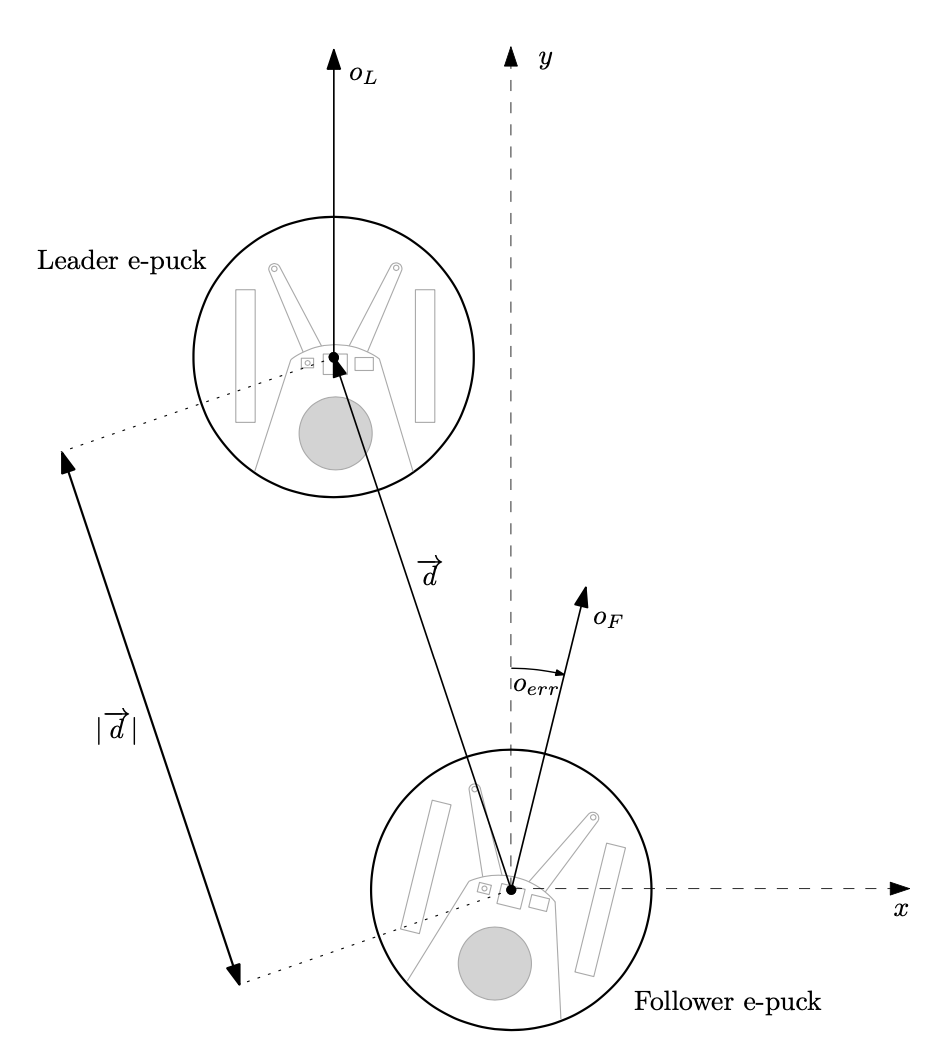
\includegraphics[width=3in]{leaderfollowerrl.png}
			%\caption{fig1}
		\end{minipage}
	}
	\subfigure[9 $\times$ 9 tile coding of state.]{
		\label{sfig:leaderfollowerrltilecoding}
		\begin{minipage}[t]{0.4\linewidth}
			\centering
			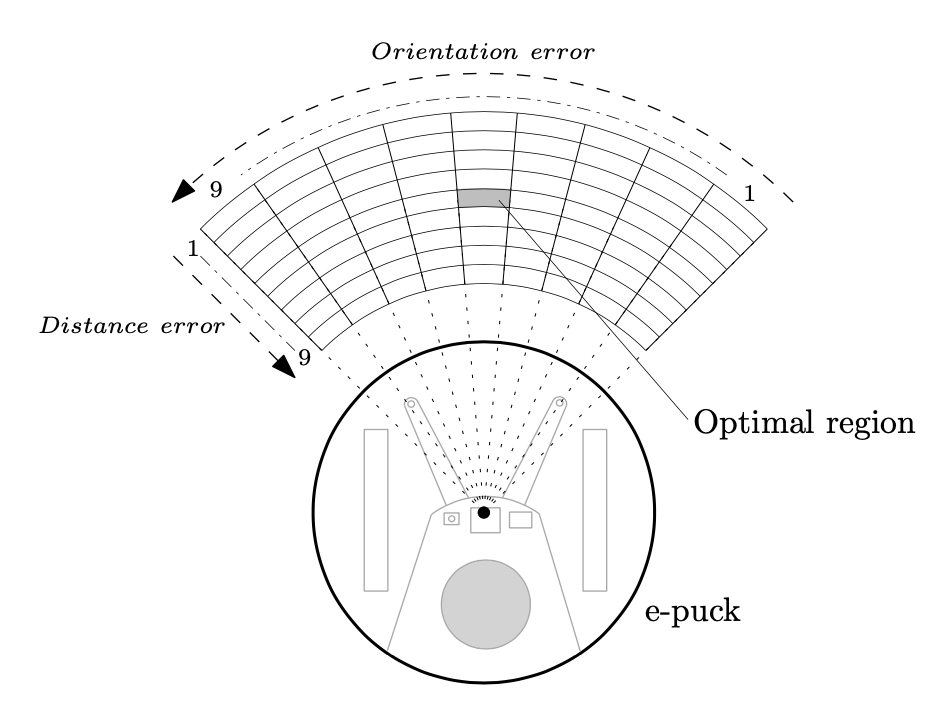
\includegraphics[width=3in]{leaderfollowerrltilecoding.png}
			%\caption{fig2}
		\end{minipage}
	}
	\caption{States and tile coding of leader-follower using RL method.}
	\label{fig:leaderfollowerrl}
\end{figure}

\subsubsection{Reinforcements}

The reinforcement process including its definition of reward function is not clearly stated is their paper.
They might use the two errors in the state to form the reward function, or there might be a specified rewarding principle in the pipeline of GQ$\lambda$ algorithm, which remains to discover.

\subsubsection{Experiment}

In their experiment, the leader agent is programmed to follow a closed circular loop , which is controlled using no learning at all, and the other agents in the group is trained to follow the agent closest in front of them.
They tested their algorithm both in the simulation and real environment.
No quantitative evaluation is provided, but only graphic results, as shown in Figure \ref{fig:leaderfollowerrlresult1} and \ref{fig:leaderfollowerrlresult2}.

\begin{figure}
	\centering
	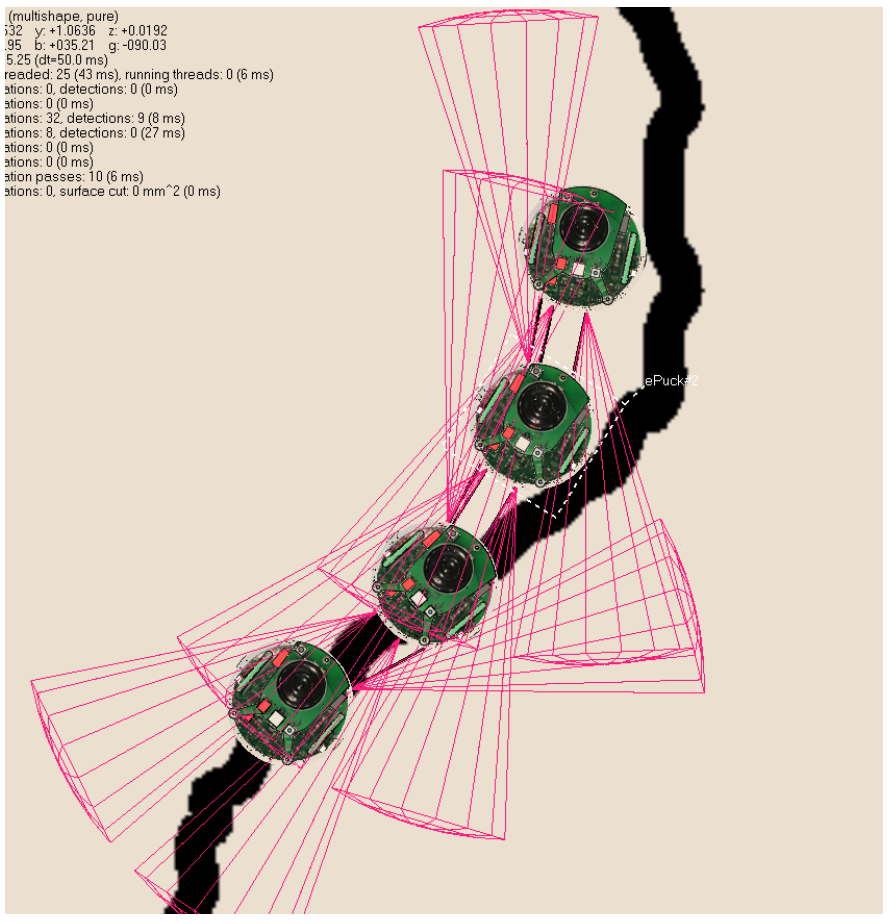
\includegraphics[width=5in]{leaderfollowerrlresult1.png}
	\caption{Simple four agent line formation in V-REP,: the first leader can be found in the lower left corner. The red cones are showing active proximity sensors.}
	\label{fig:leaderfollowerrlresult1} 
\end{figure}

\begin{figure}
	\centering
	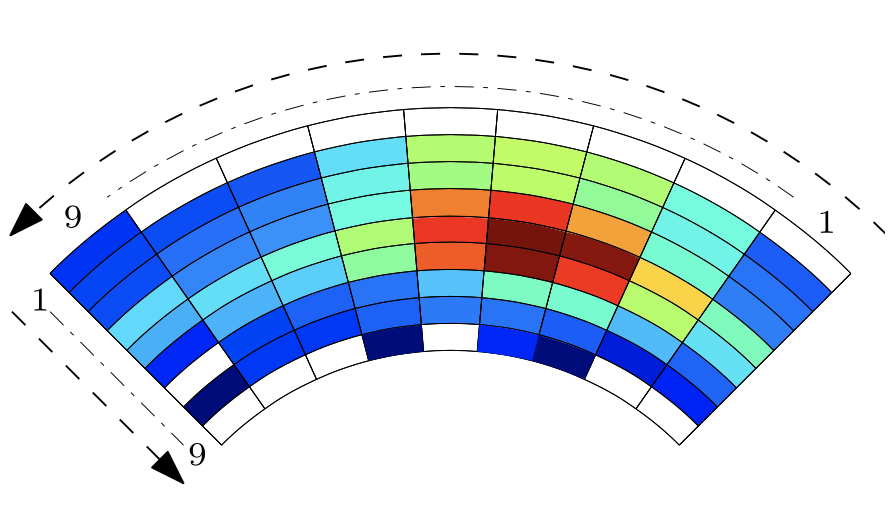
\includegraphics[width=5in]{leaderfollowerlresult2.png}
	\caption{Distribution of visited states at around 1.3 million steps. In 74\% of all cases, the leader was detected in the dark red area right to our optimal region. It stayed within the orange/red 3×3 area on the right side of the optimal region in 98.7\% of the time. To make the rarely visited states discernible, a logarithmic scale is used: red and orange values are in the range of 30\%–1\%, green values are at around 0.1\%, and blue values are another magnitude below that. The non-colored states were never visited in this experiment.}
	\label{fig:leaderfollowerrlresult2} 
\end{figure}

\subsubsection{Discussion}

In this work, the sensor setting is more practical.
Detection of agents in front of the current agents is a well developped technique, which can be done by a variaty of sensors, e.g. lidar or camera.
Also, tile coding is a good method to discretize state and action space.
Some shortcomings can also be summarised:

\begin{compactenum}
	\item This work only explored how to design a leader-follower controller by reinforcement learning, but other formation shapes and maintenance strategy is not considered.
	\item Also, environment obstacles either static or dynamic are ignored.
\end{compactenum}

And they have their research updated in \cite{aykin2018deep}. In this updated work, they use DQN instead of GQ($\lambda$), and take images as input.